% Gerado por src/prisma_counts.py -- não editar à mão; rode o script de novo.
\documentclass[border=6pt]{standalone}
\usepackage[T1]{fontenc}
\usepackage[utf8]{inputenc}
\usepackage[scaled]{helvet}
\renewcommand{\familydefault}{\sfdefault}
\usepackage{tikz}
\usetikzlibrary{positioning,calc}
\definecolor{azulborda}{RGB}{79,129,189}
\definecolor{azulaba}{RGB}{91,155,213}
\definecolor{laranja}{RGB}{247,184,38}
\begin{document}
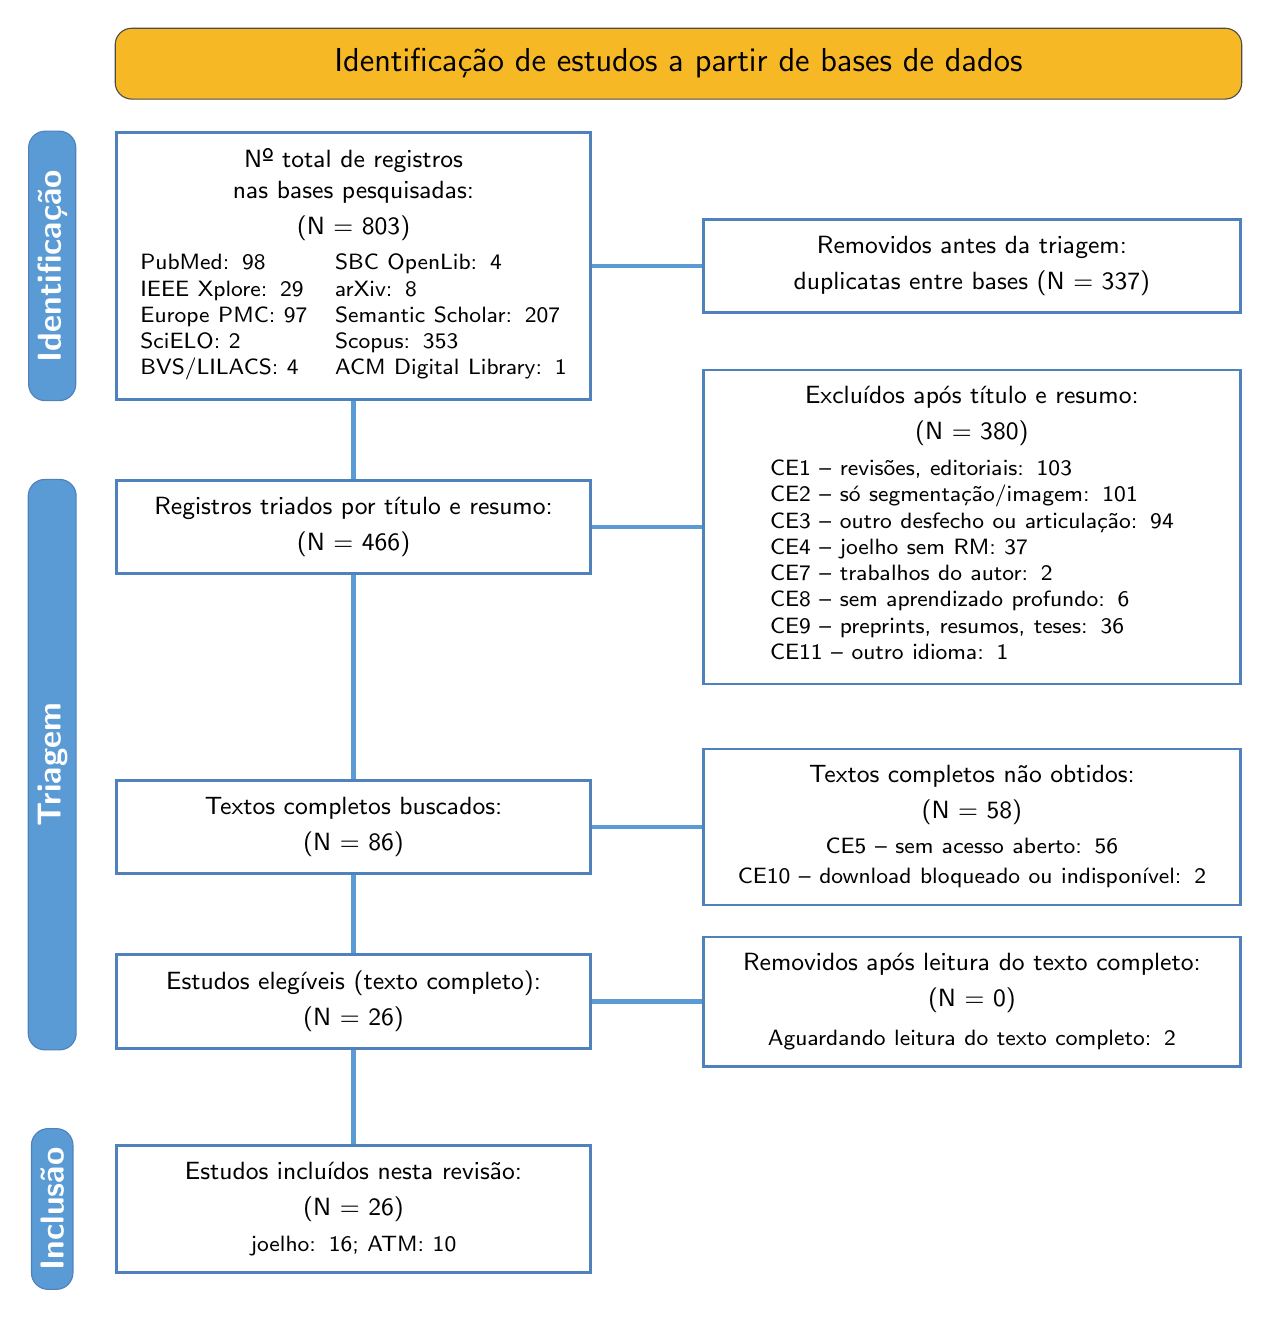
\begin{tikzpicture}[font=\small,
  caixa/.style={draw=azulborda, line width=0.9pt, fill=white, align=center, text width=5.6cm, inner sep=6pt},
  lado/.style={draw=azulborda, line width=0.9pt, fill=white, align=center, text width=6.4cm, inner sep=6pt},
  linha/.style={draw=azulaba, line width=1.6pt},
  aba/.style={draw=azulborda, fill=azulaba, rounded corners=6pt, text=white, font=\bfseries\large, minimum width=0.9cm}]
\node[caixa] (id) at (0,0) {Nº total de registros nas bases pesquisadas:\\[2pt] (N = 803)\\[3pt]
  {\footnotesize \begin{tabular}{@{}l@{\hspace{10pt}}l@{}}PubMed: 98 & SBC OpenLib: 4 \\ IEEE Xplore: 29 & arXiv: 8 \\ Europe PMC: 97 & Semantic Scholar: 207 \\ SciELO: 2 & Scopus: 353 \\ BVS/LILACS: 4 & ACM Digital Library: 1\end{tabular}}};
\node[lado, right=1.4cm of id] (dup) {Removidos antes da triagem:\\[2pt] duplicatas entre bases (N = 337)};
\node[caixa, below=1.0cm of id] (tri) {Registros triados por título e resumo:\\[2pt] (N = 466)};
\node[lado, right=1.4cm of tri] (ex1) {Excluídos após título e resumo:\\[2pt] (N = 380)\\[3pt]
  {\footnotesize \begin{tabular}{@{}l@{}}CE1 -- revisões, editoriais: 103 \\ CE2 -- só segmentação/imagem: 101 \\ CE3 -- outro desfecho ou articulação: 94 \\ CE4 -- joelho sem RM: 37 \\ CE7 -- trabalhos do autor: 2 \\ CE8 -- sem aprendizado profundo: 6 \\ CE9 -- preprints, resumos, teses: 36 \\ CE11 -- outro idioma: 1\end{tabular}}};
\node[caixa, below=2.6cm of tri] (bus) {Textos completos buscados:\\[2pt] (N = 86)};
\node[lado, right=1.4cm of bus] (ce5) {Textos completos não obtidos:\\[2pt] (N = 58)\\[3pt]
  {\footnotesize CE5 -- sem acesso aberto: 56\\ CE10 -- download bloqueado ou indisponível: 2}};
\node[caixa, below=1.0cm of bus] (ele) {Estudos elegíveis (texto completo):\\[2pt] (N = 26)};
\node[lado, right=1.4cm of ele] (ex2) {Removidos após leitura do texto completo:\\[2pt] (N = 0)\\[3pt]
  {\footnotesize Aguardando leitura do texto completo: 2}};
\node[caixa, below=1.2cm of ele] (inc) {Estudos incluídos nesta revisão:\\[2pt] (N = 26)\\[2pt]
  {\footnotesize joelho: 16; ATM: 10}};
\path let \p1=(id.north west), \p2=(dup.north east) in node[draw=black!70, fill=laranja, rounded corners=6pt,
  minimum width=\x2-\x1, minimum height=0.9cm, font=\large, anchor=south] (banner) at (\x1/2+\x2/2, \y1+0.4cm)
  {Identificação de estudos a partir de bases de dados};
\foreach \a/\b in {id/tri, tri/bus, bus/ele, ele/inc} \draw[linha] (\a) -- (\b);
\foreach \a/\b in {id/dup, tri/ex1, bus/ce5, ele/ex2} \draw[linha] (\a) -- (\b);
\path let \p1=(id.north), \p2=(id.south) in node[aba, rotate=90, minimum width=\y1-\y2] at ($(id.west)+(-0.8,0)$) {Identificação};
\path let \p1=(tri.north), \p2=(ele.south) in node[aba, rotate=90, minimum width=\y1-\y2] at ($(tri.north west)!0.5!(ele.south west)+(-0.8,0)$) {Triagem};
\path let \p1=(inc.north), \p2=(inc.south) in node[aba, rotate=90, minimum width=\y1-\y2+0.4cm] at ($(inc.west)+(-0.8,0)$) {Inclusão};
% A lista de bases não executadas vai na legenda da figura (texto), não dentro do fluxograma.
\end{tikzpicture}
\end{document}
